\twocolumn
\begin{center}
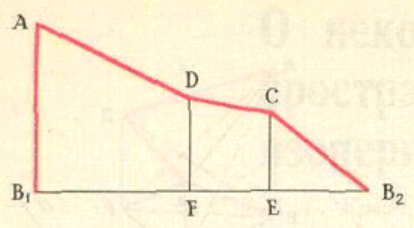
\includegraphics[width=190px]{pic1.png}
\end{center}

\noindent Рис. 4
\newline


\par \noindent $AD$ (рис. 3) выбрать так, чтобы площадь треугольника $BEF$ оказалась наибольшей из возможных.


\par Чтобы добиться этого, позаботимся сначала о том, чтобы его периметр был наибольшим. Развернем на плоскость грани\\ $ABFD$, $FDCE$, $CEB$, проектирующие четырехугольник $ABCD$ на плоскость П. В получившейся плоской фигуре (рис. 4) длина стороны $B_{1}B_{2}$ равна периметру треугольника $BFE$, откуда ясно, что этот периметр будет наибольшим в том случае, когда отрезки $AD$, $DC$, $CB$ образуют один и тот же угол $\alpha = \arccos{\frac{h}{2p-h}}$ со стороной $AB$ (рис. 5). Таким образом, пространственный четырехугольник со стороной $AB = h$ и периметром $2p$, для которого треугольник $BEF$ имеет наибольший периметр, можно получить в результате следующего построения: прямоугольник со стороной $AB_{1} = h$ и диагональю $AB_{2} = 2p - h$ сворачивается в треугольную призму так, что точки $B_{1}$ и $B_{2}$ совпадают, а ее боковым ребром служит отрезок $AB_{1}$. При этом линия $B_{1}ADCB_{2}$ превратится в искомый пространственный четырехугольник.


\begin{center}
\тз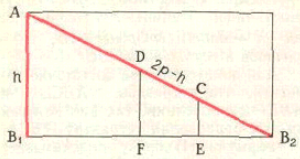
\includegraphics[width=190px]{pic2.png}
\end{center}
\noindent Рис. 5
\pagebreak

\par Таким образом, наша задача свелась к изопериметрической задаче для треугольника $BEF$. Как мы знаем, при заданном периметре  площадь этого треугольника максимальна, когда $BF = FE = EB$, вследствие чего у четырехугольника $ABCD$, являющегося решением задачи $2^\prime$, стороны $AD$, $DC$ и $CB$ равны. Этими условиями и тем, что $AD$, $DC$ и $CB$ образуют один и тот же угол с $AB$, четырехугольник $ABCD$ определяется однозначно.

\par Итак, доказана.
\par Т е о р е м а\quad2. \textit{Среди всех тетраэдров, натянутых на пространственные четырехугольники $ABCD$ с заданными периметром $2p$ и длиной $h$ стороны $AB$, наибольший объем имеет тетраэдр, натянутый на четырехугольник, стороны которого $AD$, $DC$ и $CB$ имеют равные длины и образуют равные углы со стороной $AB$.}
\par Одновременно получен способ построения экстремального четырехугольника: для этого нужно прямоугольник, у которого одна сторона равна $h$, а диагональ равна $2p - h$, свернуть в правильную треугольную призму.

\par \noindent Р е ш е н и е \quad з а д а ч и\quad3
\par Подсчитаем максимальный объем, о котором идет речь в теореме 2. Из рисунка 5 мы видим, что периметр треугольника $BFE$ равен $\sqrt{(2p-h)^{2} - h^{2}} = 2\sqrt{p(p-h)}$, а значит, его наибольшая площадь равна
\[\left[ \frac{2\sqrt{p\,(p - h)}}{3} \right]^{2}\frac{\sqrt{3}}{4} = \frac{p\,(p - h)}{3\,\sqrt{3}};\]
наконец, наибольший объем натянутого тетраэдра, в соответствии с формулой (1), равен
\begin{equation} \tag{2}
V = \frac{1}{3}\,h\,\frac{p\,(p - h)}{3\,\sqrt{3}} = \frac{p}{9\,\sqrt{3}}\,h\,(p - h)
\end{equation}

\par Теперь легко решается задача 3. Она отличается от задачи $2^\prime$ тем, что в ней задается \textit{только периметр} четырехугольника.